% Editable source for result.pdf, written by make_figures.py from run_github_38862448935/panel/result.json
\documentclass[tikz,border=6pt]{standalone}
\usepackage[T1]{fontenc}
\begin{document}
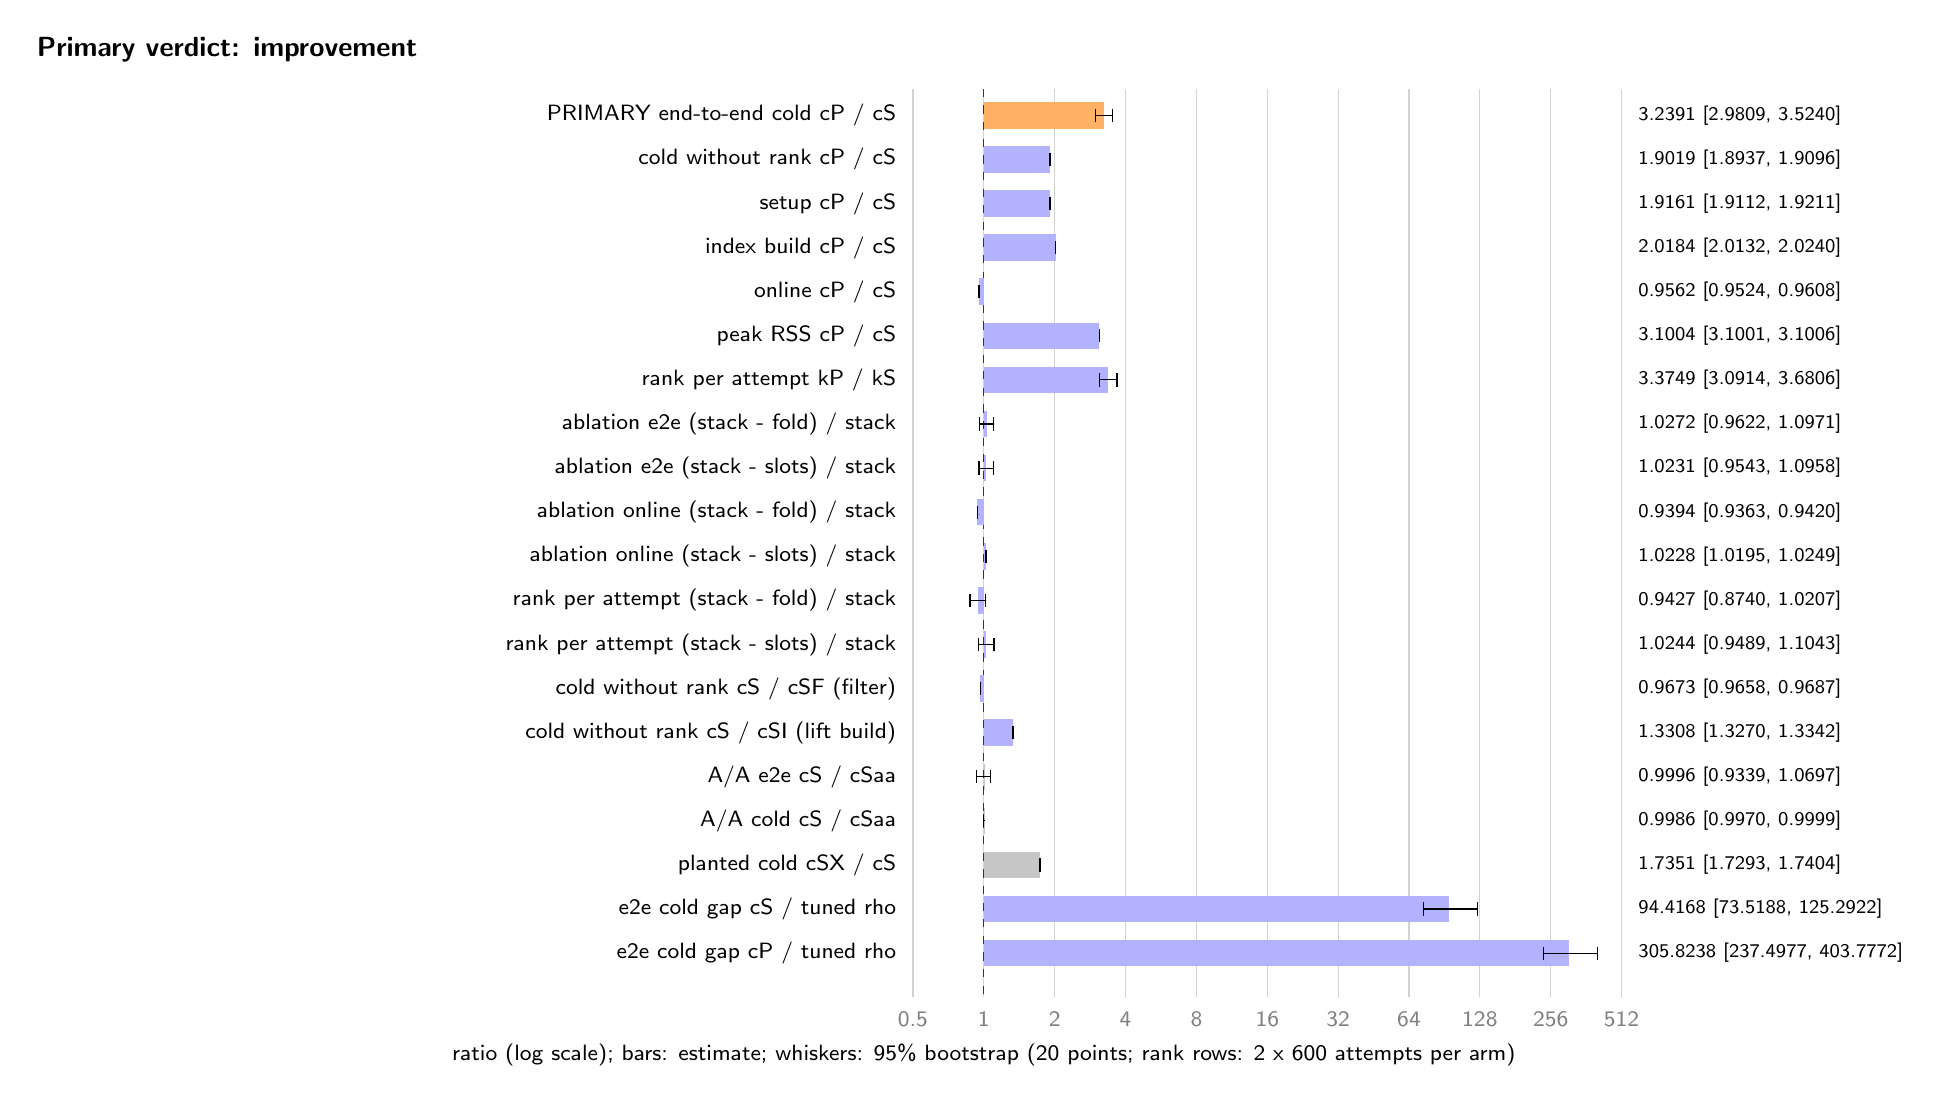
\begin{tikzpicture}[font=\sffamily\footnotesize,x=9mm,y=-5.6mm]
\draw[gray!35] (-1.0000,-0.6) -- (-1.0000,20); \node[gray] at (-1.0000,20.5) {0.5};
\draw[gray!35] (0.0000,-0.6) -- (0.0000,20); \node[gray] at (0.0000,20.5) {1};
\draw[gray!35] (1.0000,-0.6) -- (1.0000,20); \node[gray] at (1.0000,20.5) {2};
\draw[gray!35] (2.0000,-0.6) -- (2.0000,20); \node[gray] at (2.0000,20.5) {4};
\draw[gray!35] (3.0000,-0.6) -- (3.0000,20); \node[gray] at (3.0000,20.5) {8};
\draw[gray!35] (4.0000,-0.6) -- (4.0000,20); \node[gray] at (4.0000,20.5) {16};
\draw[gray!35] (5.0000,-0.6) -- (5.0000,20); \node[gray] at (5.0000,20.5) {32};
\draw[gray!35] (6.0000,-0.6) -- (6.0000,20); \node[gray] at (6.0000,20.5) {64};
\draw[gray!35] (7.0000,-0.6) -- (7.0000,20); \node[gray] at (7.0000,20.5) {128};
\draw[gray!35] (8.0000,-0.6) -- (8.0000,20); \node[gray] at (8.0000,20.5) {256};
\draw[gray!35] (9.0000,-0.6) -- (9.0000,20); \node[gray] at (9.0000,20.5) {512};
\draw[red!70!black,dashed] (0,-0.6) -- (0,20);
\node at (0,21.3) {ratio (log scale); bars: estimate; whiskers: 95\% bootstrap (20 points; rank rows: 2 x 600 attempts per arm)};
\node[anchor=west,font=\sffamily\bfseries] at (-13.5,-1.5) {Primary verdict: improvement};
\node[anchor=east] at (-1.1000,0) {PRIMARY end-to-end cold cP / cS};
\fill[orange!60] (0,-0.300000) rectangle (1.6956,0.300000);
\draw (1.5758,0) -- (1.8172,0); \draw (1.5758,-0.150000) -- (1.5758,0.150000); \draw (1.8172,-0.150000) -- (1.8172,0.150000);
\node[anchor=west,font=\sffamily\scriptsize] at (9.1000,0) {3.2391 [2.9809, 3.5240]};
\node[anchor=east] at (-1.1000,1) {cold without rank cP / cS};
\fill[blue!30] (0,0.700000) rectangle (0.9274,1.300000);
\draw (0.9212,1) -- (0.9333,1); \draw (0.9212,0.850000) -- (0.9212,1.150000); \draw (0.9333,0.850000) -- (0.9333,1.150000);
\node[anchor=west,font=\sffamily\scriptsize] at (9.1000,1) {1.9019 [1.8937, 1.9096]};
\node[anchor=east] at (-1.1000,2) {setup cP / cS};
\fill[blue!30] (0,1.700000) rectangle (0.9382,2.300000);
\draw (0.9345,2) -- (0.9420,2); \draw (0.9345,1.850000) -- (0.9345,2.150000); \draw (0.9420,1.850000) -- (0.9420,2.150000);
\node[anchor=west,font=\sffamily\scriptsize] at (9.1000,2) {1.9161 [1.9112, 1.9211]};
\node[anchor=east] at (-1.1000,3) {index build cP / cS};
\fill[blue!30] (0,2.700000) rectangle (1.0132,3.300000);
\draw (1.0095,3) -- (1.0172,3); \draw (1.0095,2.850000) -- (1.0095,3.150000); \draw (1.0172,2.850000) -- (1.0172,3.150000);
\node[anchor=west,font=\sffamily\scriptsize] at (9.1000,3) {2.0184 [2.0132, 2.0240]};
\node[anchor=east] at (-1.1000,4) {online cP / cS};
\fill[blue!30] (0,3.700000) rectangle (-0.0645,4.300000);
\draw (-0.0703,4) -- (-0.0576,4); \draw (-0.0703,3.850000) -- (-0.0703,4.150000); \draw (-0.0576,3.850000) -- (-0.0576,4.150000);
\node[anchor=west,font=\sffamily\scriptsize] at (9.1000,4) {0.9562 [0.9524, 0.9608]};
\node[anchor=east] at (-1.1000,5) {peak RSS cP / cS};
\fill[blue!30] (0,4.700000) rectangle (1.6324,5.300000);
\draw (1.6323,5) -- (1.6326,5); \draw (1.6323,4.850000) -- (1.6323,5.150000); \draw (1.6326,4.850000) -- (1.6326,5.150000);
\node[anchor=west,font=\sffamily\scriptsize] at (9.1000,5) {3.1004 [3.1001, 3.1006]};
\node[anchor=east] at (-1.1000,6) {rank per attempt kP / kS};
\fill[blue!30] (0,5.700000) rectangle (1.7548,6.300000);
\draw (1.6283,6) -- (1.8799,6); \draw (1.6283,5.850000) -- (1.6283,6.150000); \draw (1.8799,5.850000) -- (1.8799,6.150000);
\node[anchor=west,font=\sffamily\scriptsize] at (9.1000,6) {3.3749 [3.0914, 3.6806]};
\node[anchor=east] at (-1.1000,7) {ablation e2e (stack - fold) / stack};
\fill[blue!30] (0,6.700000) rectangle (0.0387,7.300000);
\draw (-0.0556,7) -- (0.1338,7); \draw (-0.0556,6.850000) -- (-0.0556,7.150000); \draw (0.1338,6.850000) -- (0.1338,7.150000);
\node[anchor=west,font=\sffamily\scriptsize] at (9.1000,7) {1.0272 [0.9622, 1.0971]};
\node[anchor=east] at (-1.1000,8) {ablation e2e (stack - slots) / stack};
\fill[blue!30] (0,7.700000) rectangle (0.0330,8.300000);
\draw (-0.0675,8) -- (0.1319,8); \draw (-0.0675,7.850000) -- (-0.0675,8.150000); \draw (0.1319,7.850000) -- (0.1319,8.150000);
\node[anchor=west,font=\sffamily\scriptsize] at (9.1000,8) {1.0231 [0.9543, 1.0958]};
\node[anchor=east] at (-1.1000,9) {ablation online (stack - fold) / stack};
\fill[blue!30] (0,8.700000) rectangle (-0.0902,9.300000);
\draw (-0.0949,9) -- (-0.0862,9); \draw (-0.0949,8.850000) -- (-0.0949,9.150000); \draw (-0.0862,8.850000) -- (-0.0862,9.150000);
\node[anchor=west,font=\sffamily\scriptsize] at (9.1000,9) {0.9394 [0.9363, 0.9420]};
\node[anchor=east] at (-1.1000,10) {ablation online (stack - slots) / stack};
\fill[blue!30] (0,9.700000) rectangle (0.0326,10.300000);
\draw (0.0278,10) -- (0.0355,10); \draw (0.0278,9.850000) -- (0.0278,10.150000); \draw (0.0355,9.850000) -- (0.0355,10.150000);
\node[anchor=west,font=\sffamily\scriptsize] at (9.1000,10) {1.0228 [1.0195, 1.0249]};
\node[anchor=east] at (-1.1000,11) {rank per attempt (stack - fold) / stack};
\fill[blue!30] (0,10.700000) rectangle (-0.0851,11.300000);
\draw (-0.1942,11) -- (0.0296,11); \draw (-0.1942,10.850000) -- (-0.1942,11.150000); \draw (0.0296,10.850000) -- (0.0296,11.150000);
\node[anchor=west,font=\sffamily\scriptsize] at (9.1000,11) {0.9427 [0.8740, 1.0207]};
\node[anchor=east] at (-1.1000,12) {rank per attempt (stack - slots) / stack};
\fill[blue!30] (0,11.700000) rectangle (0.0348,12.300000);
\draw (-0.0757,12) -- (0.1432,12); \draw (-0.0757,11.850000) -- (-0.0757,12.150000); \draw (0.1432,11.850000) -- (0.1432,12.150000);
\node[anchor=west,font=\sffamily\scriptsize] at (9.1000,12) {1.0244 [0.9489, 1.1043]};
\node[anchor=east] at (-1.1000,13) {cold without rank cS / cSF (filter)};
\fill[blue!30] (0,12.700000) rectangle (-0.0480,13.300000);
\draw (-0.0503,13) -- (-0.0459,13); \draw (-0.0503,12.850000) -- (-0.0503,13.150000); \draw (-0.0459,12.850000) -- (-0.0459,13.150000);
\node[anchor=west,font=\sffamily\scriptsize] at (9.1000,13) {0.9673 [0.9658, 0.9687]};
\node[anchor=east] at (-1.1000,14) {cold without rank cS / cSI (lift build)};
\fill[blue!30] (0,13.700000) rectangle (0.4123,14.300000);
\draw (0.4082,14) -- (0.4159,14); \draw (0.4082,13.850000) -- (0.4082,14.150000); \draw (0.4159,13.850000) -- (0.4159,14.150000);
\node[anchor=west,font=\sffamily\scriptsize] at (9.1000,14) {1.3308 [1.3270, 1.3342]};
\node[anchor=east] at (-1.1000,15) {A/A e2e cS / cSaa};
\fill[gray!45] (0,14.700000) rectangle (-0.0005,15.300000);
\draw (-0.0987,15) -- (0.0973,15); \draw (-0.0987,14.850000) -- (-0.0987,15.150000); \draw (0.0973,14.850000) -- (0.0973,15.150000);
\node[anchor=west,font=\sffamily\scriptsize] at (9.1000,15) {0.9996 [0.9339, 1.0697]};
\node[anchor=east] at (-1.1000,16) {A/A cold cS / cSaa};
\fill[gray!45] (0,15.700000) rectangle (-0.0021,16.300000);
\draw (-0.0044,16) -- (-0.0001,16); \draw (-0.0044,15.850000) -- (-0.0044,16.150000); \draw (-0.0001,15.850000) -- (-0.0001,16.150000);
\node[anchor=west,font=\sffamily\scriptsize] at (9.1000,16) {0.9986 [0.9970, 0.9999]};
\node[anchor=east] at (-1.1000,17) {planted cold cSX / cS};
\fill[gray!45] (0,16.700000) rectangle (0.7950,17.300000);
\draw (0.7902,17) -- (0.7994,17); \draw (0.7902,16.850000) -- (0.7902,17.150000); \draw (0.7994,16.850000) -- (0.7994,17.150000);
\node[anchor=west,font=\sffamily\scriptsize] at (9.1000,17) {1.7351 [1.7293, 1.7404]};
\node[anchor=east] at (-1.1000,18) {e2e cold gap cS / tuned rho};
\fill[blue!30] (0,17.700000) rectangle (6.5610,18.300000);
\draw (6.2000,18) -- (6.9692,18); \draw (6.2000,17.850000) -- (6.2000,18.150000); \draw (6.9692,17.850000) -- (6.9692,18.150000);
\node[anchor=west,font=\sffamily\scriptsize] at (9.1000,18) {94.4168 [73.5188, 125.2922]};
\node[anchor=east] at (-1.1000,19) {e2e cold gap cP / tuned rho};
\fill[blue!30] (0,18.700000) rectangle (8.2566,19.300000);
\draw (7.8918,19) -- (8.6574,19); \draw (7.8918,18.850000) -- (7.8918,19.150000); \draw (8.6574,18.850000) -- (8.6574,19.150000);
\node[anchor=west,font=\sffamily\scriptsize] at (9.1000,19) {305.8238 [237.4977, 403.7772]};
\end{tikzpicture}
\end{document}
